

\tikzset{every picture/.style={line width=0.75pt}} %set default line width to 0.75pt        

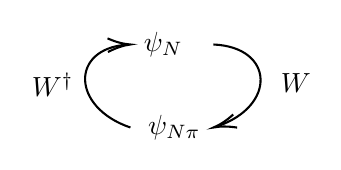
\begin{tikzpicture}[x=0.75pt,y=0.75pt,yscale=-1,xscale=1]
	%uncomment if require: \path (0,300); %set diagram left start at 0, and has height of 300
	
	%Curve Lines [id:da45911359937309637] 
	\draw    (280,60) .. controls (309.48,61.29) and (310.45,89.75) .. (281.79,99.43) ;
	\draw [shift={(280,100)}, rotate = 343.41] [color={rgb, 255:red, 0; green, 0; blue, 0 }  ][line width=0.75]    (10.93,-3.29) .. controls (6.95,-1.4) and (3.31,-0.3) .. (0,0) .. controls (3.31,0.3) and (6.95,1.4) .. (10.93,3.29)   ;
	%Curve Lines [id:da6231994153364976] 
	\draw    (240,100) .. controls (211.46,90.32) and (210.89,62.08) .. (238.29,60.09) ;
	\draw [shift={(240,60)}, rotate = 178.19] [color={rgb, 255:red, 0; green, 0; blue, 0 }  ][line width=0.75]    (10.93,-3.29) .. controls (6.95,-1.4) and (3.31,-0.3) .. (0,0) .. controls (3.31,0.3) and (6.95,1.4) .. (10.93,3.29)   ;
	
	% Text Node
	\draw (245,52.4) node [anchor=north west][inner sep=0.75pt]    {$\psi _{N}$};
	% Text Node
	\draw (247,92.4) node [anchor=north west][inner sep=0.75pt]    {$\psi _{N\pi }$};
	% Text Node
	\draw (191,72.4) node [anchor=north west][inner sep=0.75pt]    {$W^{\dagger }$};
	% Text Node
	\draw (311,72.4) node [anchor=north west][inner sep=0.75pt]    {$W$};
	
	
\end{tikzpicture}